%TODO: Раздел второй - ЭЛЕКТРОМАГНИТНЫЕ ПЕРЕХОДНЫЕ ПРОЦЕССЫ ПРИ СОХРАНЕНИИ СИММЕТРИИ ТРЕХФАЗНОЙ ЦЕПИ
\chapter{Переходный процесс в простейших трехфазных цепях}
\label{chap:3 perehodnyi_protcess_v_prosteishikh_trekhfaznykh_tcepiakh}

\section{Постановка задачи и ее ограничения}
\label{sec:3-1 postanovka_zadachi_i_ee_ogranicheniia}

Симметричную трехфазную цепь с сосредоточенными активными сопротивлениями и индуктивностями при отсутствии в ней трансформаторных связей условимся называть \so{простейшей} трехфазной цепью.

Электромагнитный переходный процесс в такой цепи рассмотрим сначала при условии, что ее питание осуществляется от источника, сопротивление которого равно нулю и его напряжение, изменяясь с постоянной частотой, имеет неизменную амплитуду\footnote{Применение чувствительного и быстродействующего автоматического регулировании возбуждения генераторов дополнительно способствует принятию указанного предположения.}. Обычно его называют источником бесконечной  мощности.

Включение в схему такого источника, вообще говоря, соответствует теоретическому пределу, когда изменение внешних условий не влияет на работу самого источнику. Практически это имеет место, например, при коротких замыканиях в относительно маломощных электрических установках или протяженных сетях, питаемых от крупных энергетических систем (см.~\colorbox{red}{гл. 17}).

С исследованием переходных процессов в подобных условиях читатель знаком из курса теоретических основ электротехники. Поэтому задачей данной главы является кратко напомнить основные выводы такого исследования, отметить особенности многофазной цепи по сравнению с однофазной, привести некоторые упрощенные приемы расчета и обратить внимание на влияние ряда факторов.

\section{Трехфазное короткое замыкание в неразветвленной цепи}
\label{sec:3-2 trekhfaznoe_korotkoe_zamykanie_v_nerazvetvlennoi_tcepi}

Обратимся к рис.~\ref{ris:3-1 simple_3_phase_circut}, на котором представлена простейшая симметричная трехфазная цепь. В ней условно принято, что на одном ее участке имеется взаимоиндукция между фазами, а на другом она отсутствует. Цепь присоединена к источнику синусоидального напряжения с неизменными амплитудой и частотой.

Рассмотрим переходный процесс, вызванный включением выключателя \textit{B}, за которым сделана закоротка, что равносильно возникновению металлического трехфазного короткого замыкания между двумя участками данной цепи.

\begin{figure}[h]
	\center{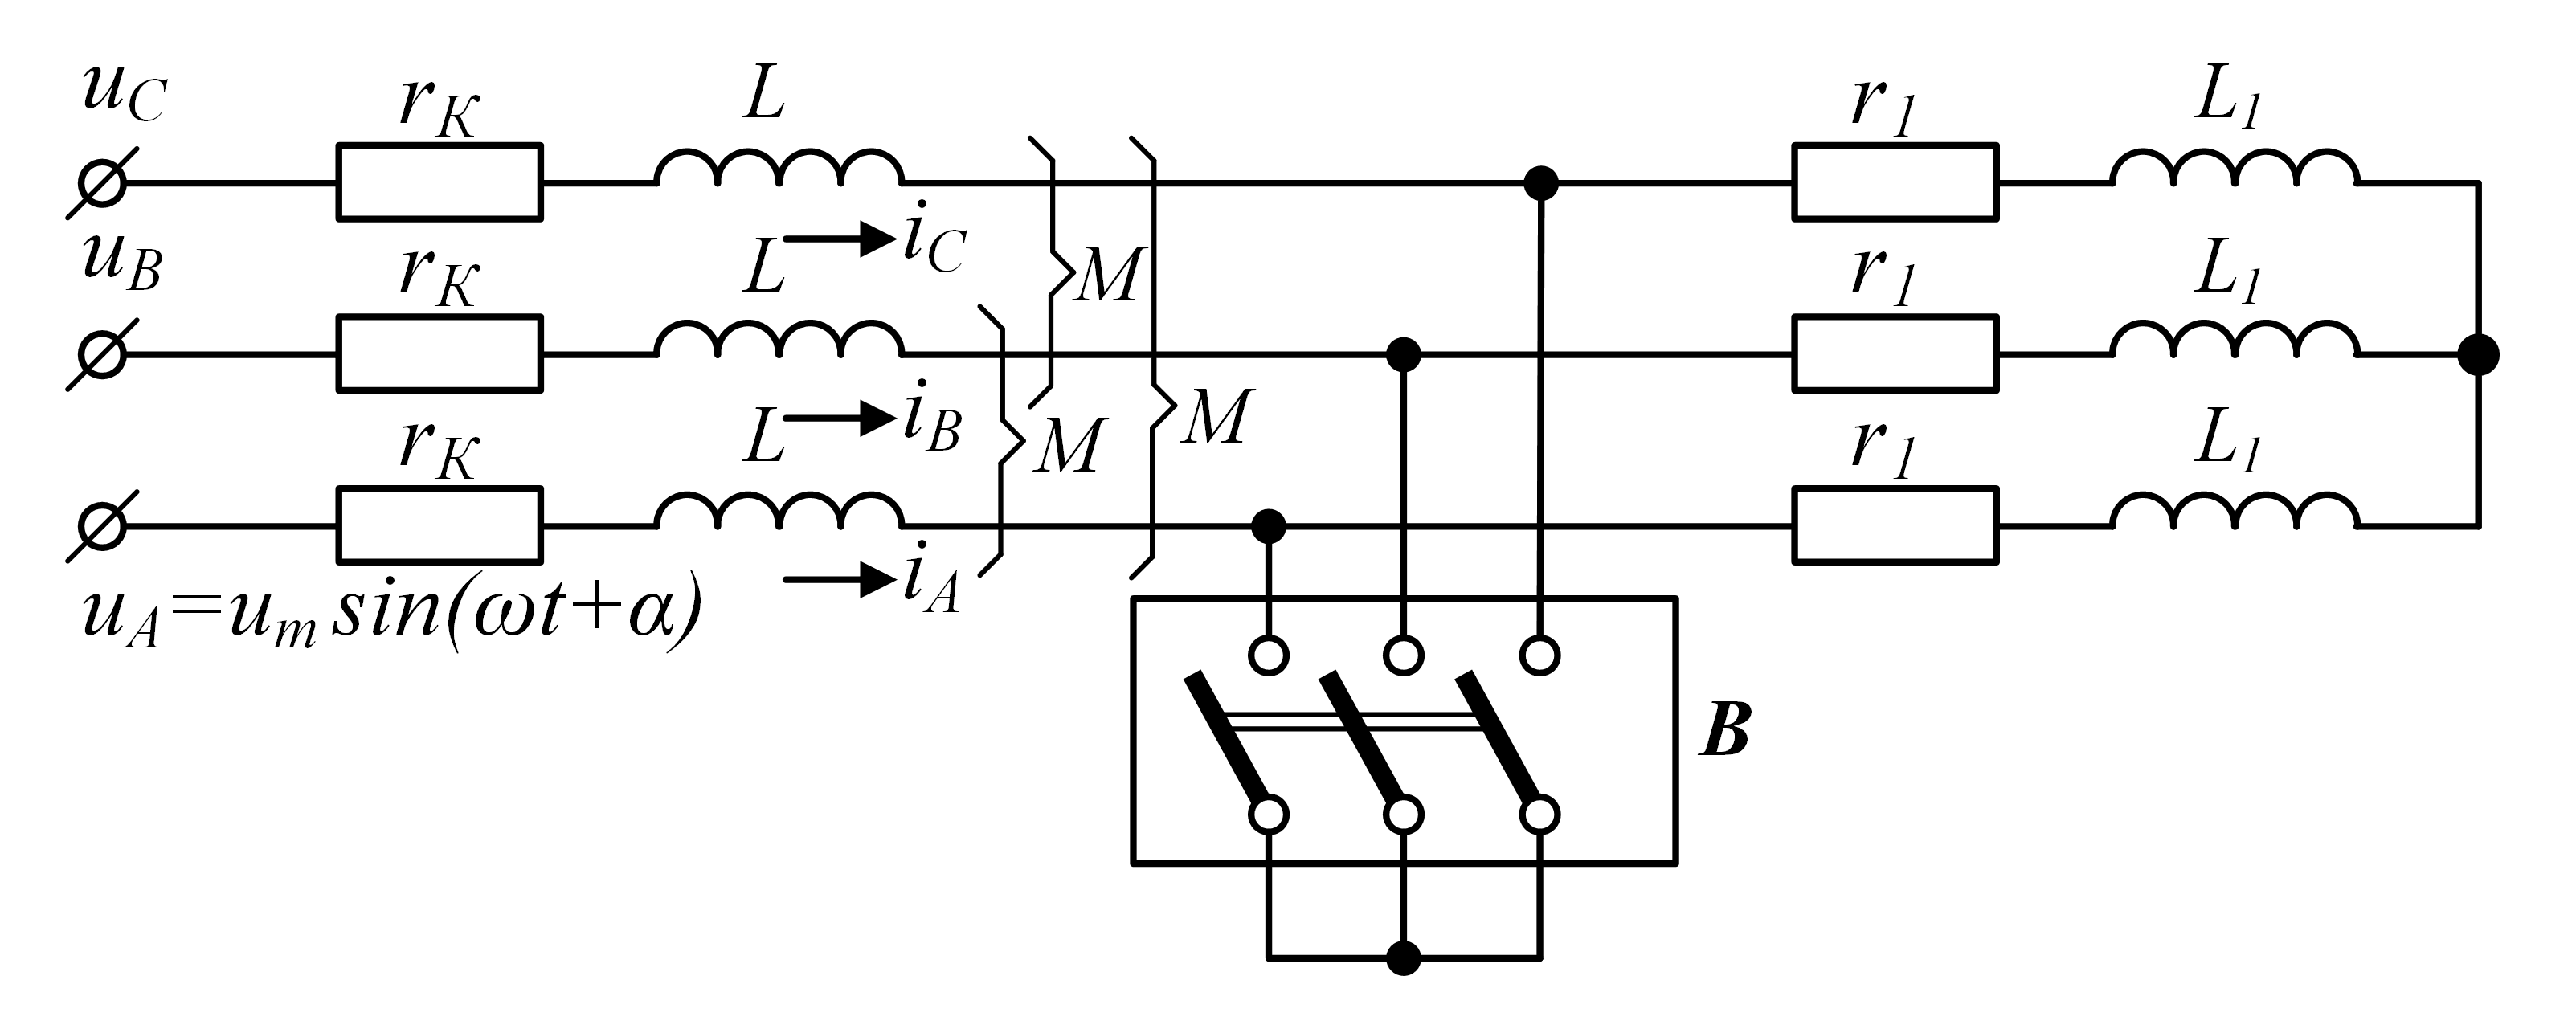
\includegraphics[width=0.9\linewidth]{pic/3-1}}
	\caption{Простейшая трехфазная электрическая цепь.}
	\label{ris:3-1 simple_3_phase_circut}
\end{figure}

Пусть векторы $ \overset{\;.}{U}_A $, $ \overset{\;.}{U}_B $, $ \overset{\;.}{U}_C $, $ \overset{\;.}{I}_A $, $ \overset{\;.}{U}_B $, $ \overset{\;.}{U}_C $ (рис. \colorbox{red}{3-2})
характеризуют предшествующий режим рассматриваемой цепи, а вертикаль \textit{tt} является неподвижной линией времени, т.~е. мгновенные значения отдельных величии определяются проекциями на эту линию соответствующих вращающихся векторов. Момент возникновения короткого замыкания будем фиксировать значением угла $ \alpha $ (т.~е. \so{фазой включения}) между вектором напряжения фазы \textit{A} и горизонталью. \colorbox{red}{(рис. 3-2)}.

После включения выключателя \textit{В} цепь рис.~\ref{ris:3-1 simple_3_phase_circut} распадается на два независимых друг от друга участка. Участок с $ r_1 $ и $ L_1 $ оказывается зашунтированным коротким замыканием и ток в нем будет поддерживаться лишь до тех пор, пока запасенная в индуктивности $ L_1 $ энергия магнитного потока не перейдет в тепло, поглощаемое активным сопротивлением $ r_1 $.

Дифференциальное уравнение равновесия в каждой фазе этого участка имеет вид:

\begin{equation}
	0 = ir_1 + L_1 \frac{di}{dt}.
	\label{eq:3-1 diff_ur}
\end{equation}

Его решение общеизвестно:

\begin{equation}
	i = i_0 e^{-t / T_{\text{а}1}}; %TODO: Проверить формулу, какая-то черка в степени
	\label{eq:3-2 diff_solve}
\end{equation}

оно показывает, что здесь имеется лишь свободный ток, который затухает по экспоненте с постоянной времени

\begin{equation}
	T_{\text{а}1} = \frac{L_1}{r_1} = \frac{x_1}{\omega r_1}, \textit{~сек}.
	\label{eq:3-3 T_a1}
\end{equation}

Начальное значение свободного тока в каждой фазе зашунтированного участка цепи, очевидно, равно предшествовавшему мгновенному значению тока, поскольку в цепи с индуктивностью не может произойти внезапного (скачком) изменения тока. В общем случае свободные токи в фазах различны, хотя их затухание, разумеется, происходит с одной и той же постоянной времени. В одной из фаз свободный ток может вообще отсутствовать, если в момент возникновения короткого замыкакия предшествовавший ток в этой фазе проходил через нуль; при этом свободные токи в двух других фазах будут одинаковы по величине, но противоположны по направлению.






